\documentclass[border=10pt]{standalone}
\usepackage{pgfplots}
%\pgfplotsset{width=7cm,compat=1.8}
\begin{document}
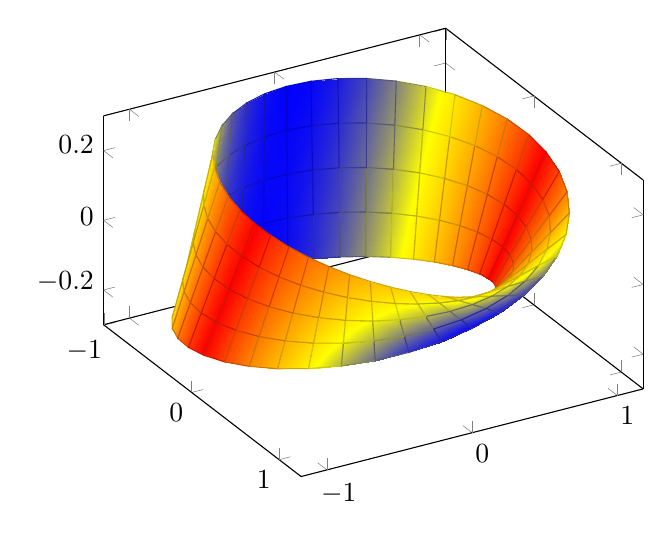
\begin{tikzpicture}
  \begin{axis}[
    %view/h=-10,
    %hide axis,
    view = {60}{40}
  ]
  \addplot3 [
    surf,
    %colormap/greenyellow,
    colormap={periodic}{
            color=(blue)
               color=(yellow)
                  color=(orange)
                     color=(red)
                  color=(orange)
               color=(yellow)
            color=(blue)},
    shader     = faceted interp,
    point meta = x,
    samples    = 40,
    samples y  = 5,
    z buffer   = sort,
    domain     = 0:360,
    y domain   =-0.5:0.5
  ] (
    {(1+0.5*y*cos(x/2)))*cos(x)},
    {(1+0.5*y*cos(x/2)))*sin(x)},
    {0.5*y*sin(x/2)}
  );

%   \addplot3 [
%     samples=50,
%     domain=-145:180, % The domain needs to be adjusted manually,
%                      % depending on the camera angle, unfortunately
%     samples y=0,
%     thick
%   ] (
%     {cos(x)},
%     {sin(x)},
%     {0}
%   );
  \end{axis}
\end{tikzpicture}
\end{document}